\chapter{Оцінка і порівняння моделей}


У ході курсової роботи для оцінки та візуалізації моделей була створена 
програма, яка дозволяє користувачу регулювати параметри та одразу бачити, 
як вони впливають на прогнози. Також реалізована кнопка, яка починає 
оптимізацїю початкових параметрів, налаштованих користувачем, методом рою 
часток (одна з часток ініціалізована початковими параметрами). Також 
є опція зберегти параметри у форматі json. 
Основна програма написана на мові програмування Python, функції поделювання 
написані на C задля збільшення швидкості оптимізації.

\begin{figure}[H]
    \centering
    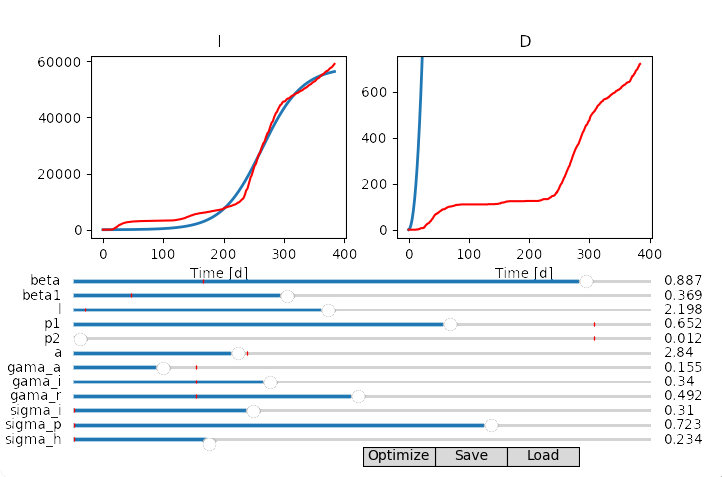
\includegraphics[scale=0.7]{program.png}
    \caption{Програма для підбору і оптимізації параметрів моделей}
    \label{fig:plot0}
\end{figure}


\section{Справжні дані та оцінка ефективності}

Прогнозувати будемо розвиток коронавірусу у Люксимбургу через те, що країна 
досить не велика та має середню густоту населення. 
Підбирати параметри будемо за перші 50 днів епідемії і відповідний прогноз 
будемо робити на наступні два тижні. 

\section{SIR}


SIR модель погано моделює навіть ту частину графіка, яку ми використали для 
налаштування її параметрів. Середня різниця між графіками на відрізку 
прогнозування (20 днів) має порядк сотень людей. 
Сумма квадратів відстаней між графіками у кожній цілій точці  
(далі будемо називати це похибкою)складає 36695055916.


\begin{figure}[H]
    \centering
    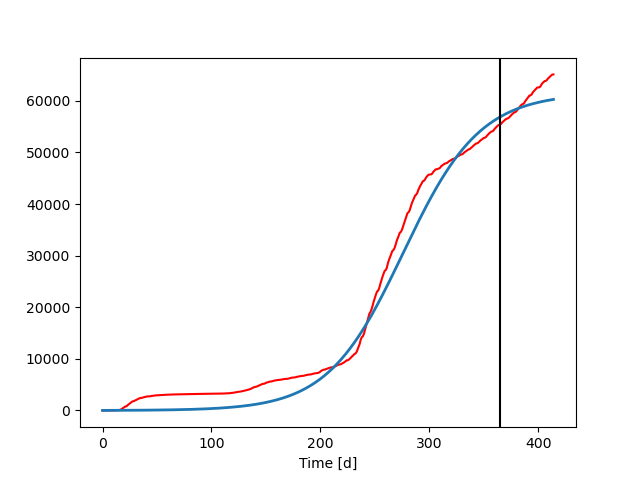
\includegraphics[scale=0.5]{SIR365.png}
    \caption{Прогноз SIR моделі після 365 днів}
    \label{fig:plot1}
\end{figure}


\section{SEIR}


З SEIR моделлю вже можливо досить непогано апроксимувати графік, проте 
прогноз і реальні дані мають зовсім різну динаміку, порядок похибки - 
тисячі, отже дану модель не можна використовувати для пронозів. 
Відстань між графіками 36695095347.


\begin{figure}[H]
    \centering
    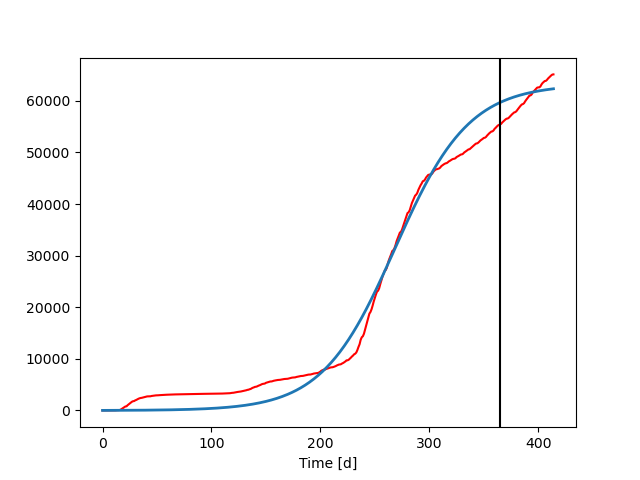
\includegraphics[scale=0.5]{SEIR365.png}
    \caption{Прогноз SEIR моделі після 365 днів}
    \label{fig:plot2}
\end{figure}
\section{SEIPR}

Модель має велику похибку на 365 день моделювання, через це прогноз 
на наступні дні має велику різницю з реальними данними. 
Загальна похибка 36606095757.

\begin{figure}[H]
    \centering
    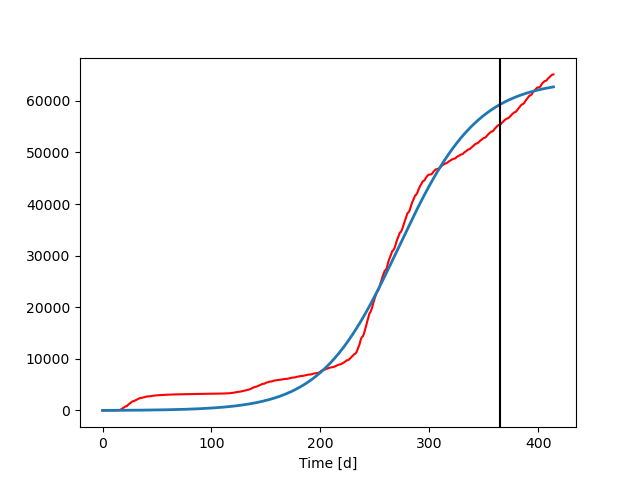
\includegraphics[scale=0.5]{SEIPR365.png}
    \caption{Прогноз SIPR моделі після 365 днів}
    \label{fig:plot3}
\end{figure}
\section{SEIAPR}

Модель краще апроксимує графік, проте все ще погано моделює 
кількість хворих на короткі періоди часу. 
Загальна похибка 36663218005
\begin{figure}[H]
    \centering
    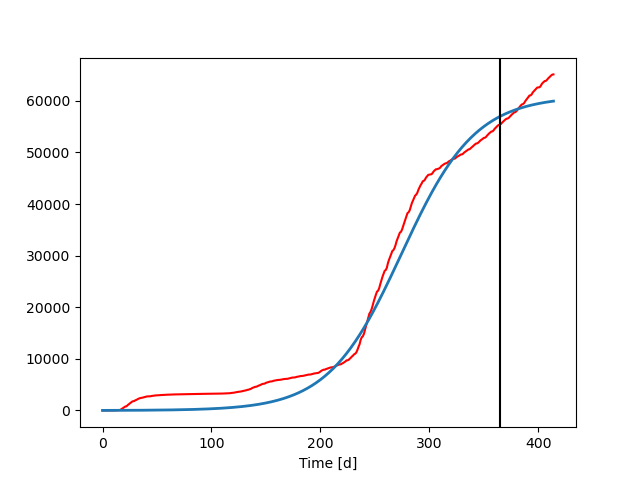
\includegraphics[scale=0.5]{SEIAPR365.png}
    \caption{Прогноз SEIAPR моделі після 365 днів}
    \label{fig:plot4}
\end{figure}
\section{SEIAPHRD}


Данна модель непогано апроксимує графік, проте початок у них досить сильно 
розбігається. Також сильно розбігаються графіки смертей та госпіталізованих.
Модель спромоглася зробити досить точний прогноз на декілька 
днів. Загальні похибка 2121522078. 
\begin{figure}[H]
    \centering
    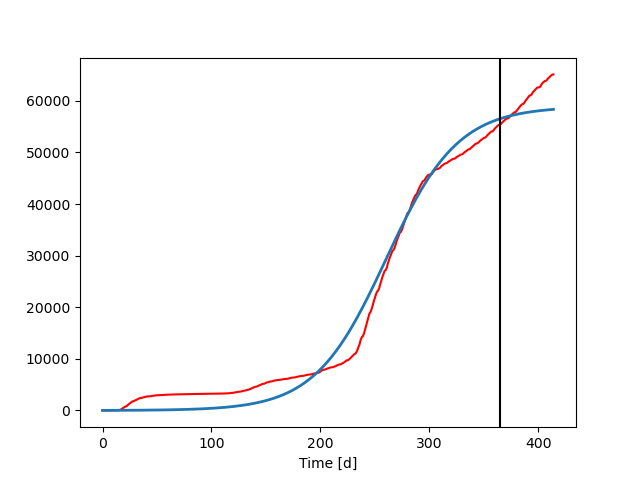
\includegraphics[scale=0.5]{model1_365.png}
    \caption{Прогноз SEIAPHRD моделі після 365 днів}
    \label{fig:plot5}
\end{figure}
\section{Порівняння моделей та результати}